\chapter{Results}
\section{Carotid Segmentation from MRA-TOF}
% GPT: fix sentencing 
As illustrated in Figure~\ref{fig:seg_compare}, the cuboid mask plays a crucial role in the carotid segmentation.
Because no ground truth segmentation is available, visual inspection was used to evaluate the results.
In Figure~\ref{TODO}, we see the 3D model of segmented ICA of a subject.
\begin{figure}[h]
	\centering
	\begin{subfigure}{0.45\textwidth}
		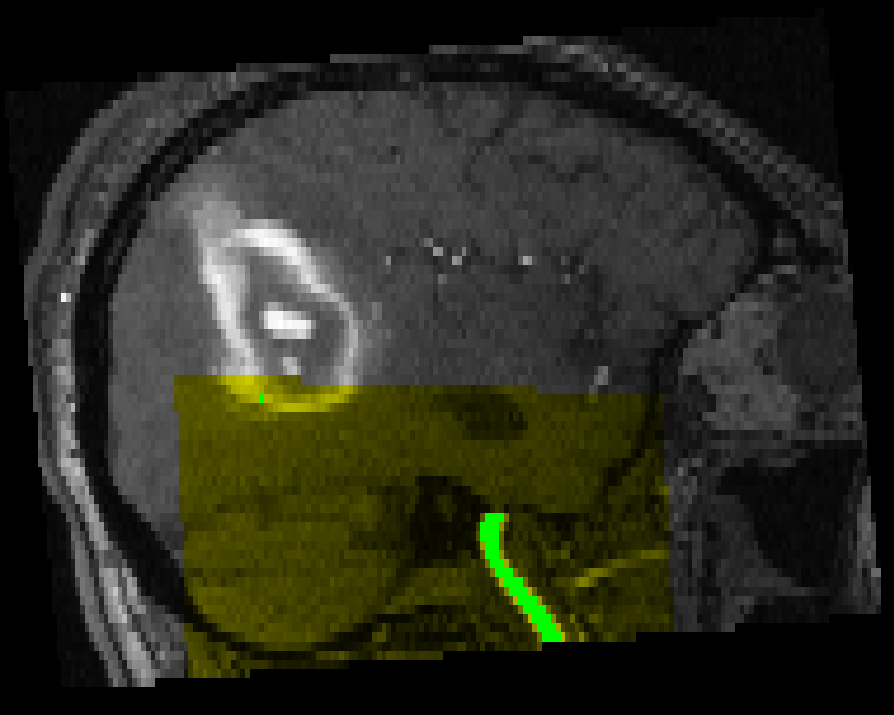
\includegraphics[width=\textwidth]{figures/molgu07704_bbox.png}
		\caption{}
		\label{subfig:seg_bbox}
	\end{subfigure}
	\begin{subfigure}{0.45\textwidth}
		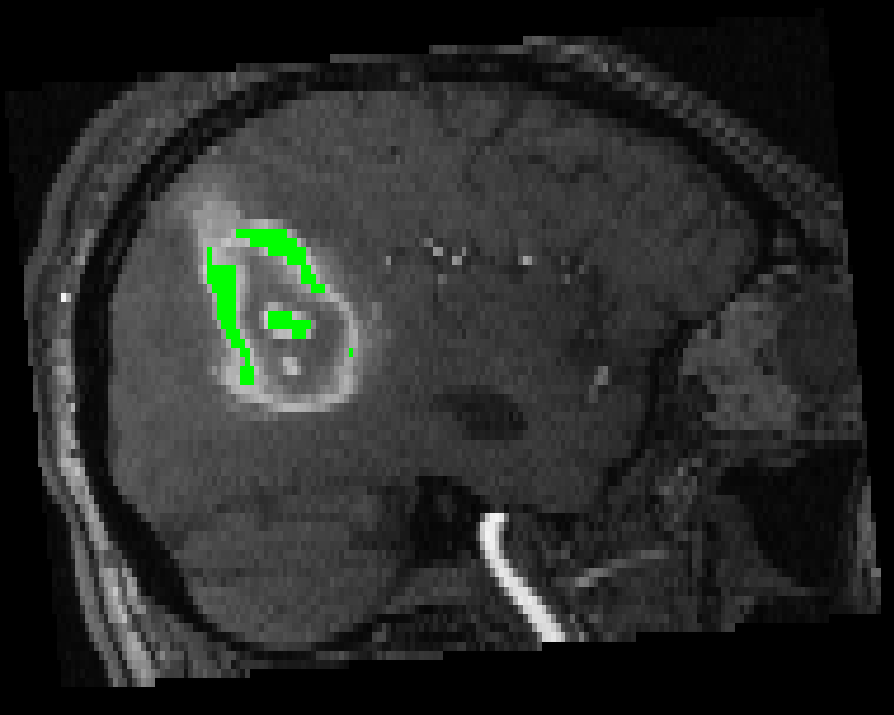
\includegraphics[width=\textwidth]{figures/molgu07704_nobbox.png}
		\caption{}
		\label{subfig:seg_nobbox}
	\end{subfigure}
	\caption{Comparison of carotid segmentation (green) with (a) and without (b) a cuboid mask (yellow). In the absence of the cuboid mask, the segmentation algorithm fails to capture the carotid and instead incorrectly identifies the brain lesion}
	\label{fig:seg_compare}
\end{figure}

\begin{figure}[t]
	\centering
	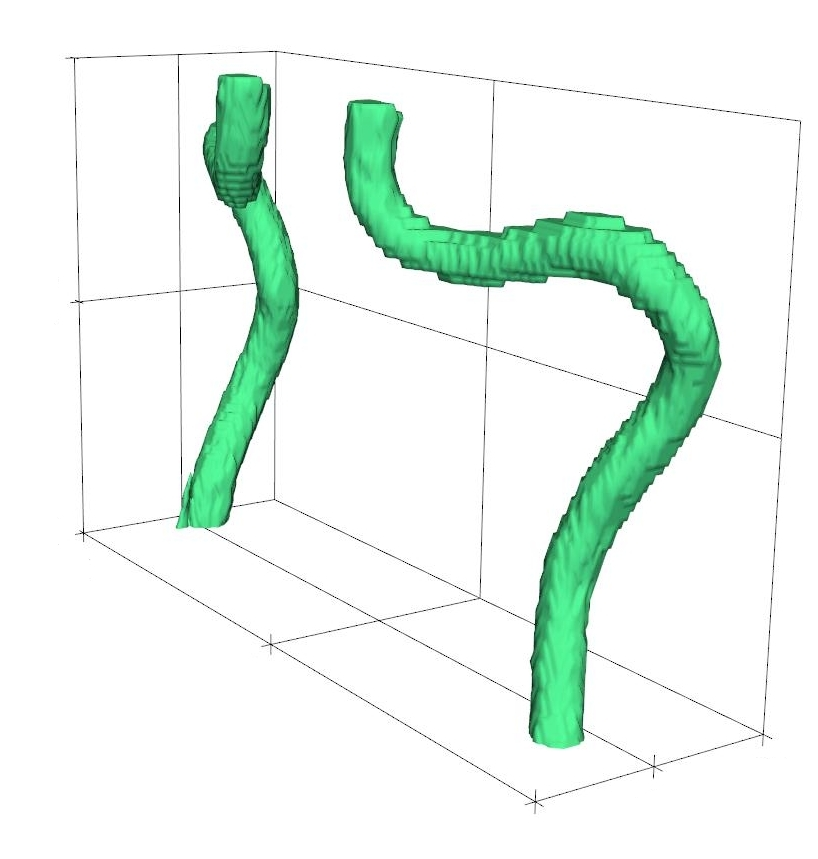
\includegraphics[width=0.4\textwidth]{figures/carotid_3d.jpg}
	\caption{3D visualization of segmented internal carotid arteries}
\end{figure}

% GPT: Hyperparameter is the correct term?
\section{Hyperparameter Tuning}
% GPT: fix sentencing and coherence
The number of principle components $p$ was chosen as 3 by analysing the explained variance ratio plot in Figure~\ref{TODO}.
We see with only 3 components we get more than 90\% explained variability.
To prove the availability of the method, we seek to find the lowest possible number of population needed for the PCA in our \fdg $\,$ dataset.
To do this, the experiment was repeated 10 times each time with a different random seed for choosing population for $N=\{5,10,15,20,30,40,50,60\}$ and the median quantification errors were compared.
As apparent in Figure~\ref{TODO}, we see a plateau in the performance after $N=20$ and it was chosen as the ideal population sample count.
For the \yohimbine$\,$ dataset since it only has 7 subjects, the maximum amount $N=6$ was chosen.


\begin{figure}[t]
	\centering
	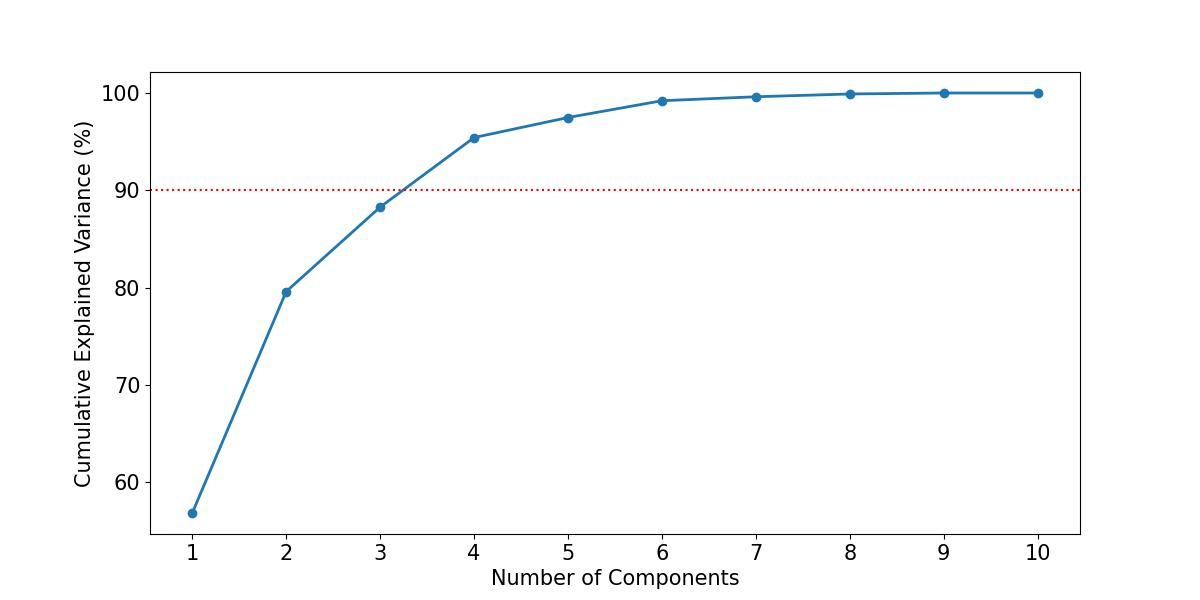
\includegraphics[width=\textwidth]{figures/pca_explained_variance.jpg}
	% gpt: add caption its the x=n components, y=cumulative explained variance % plot
	\caption{}
\end{figure}
\begin{figure}[t]
	\centering
	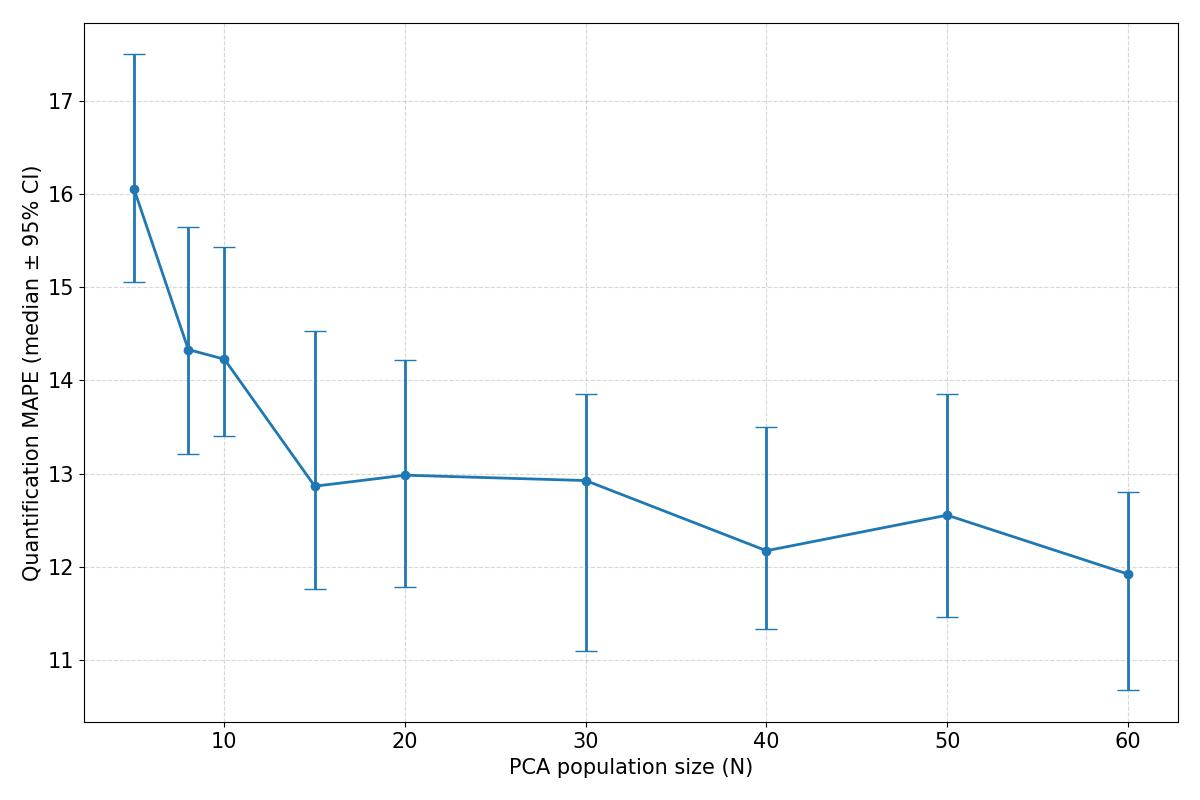
\includegraphics[width=0.8\textwidth]{figures/pca_n_experiment.jpg}
	%gpt: its the plt.xlabel("PCA population size (N)"); plt.ylabel("MAPE Quantification Error (median ± 95% CI)") errorplot
	\caption{}
\end{figure}

% GPT: fix sentencing and coherence
In classical model fitting using SA, an appropriate spectral range is chosen based on the radioisotope half-life (e.g. $10^{-4} \mathrm{s}^{-1}$ to $1 \mathrm{s}^{-1}$ for $^{18}\mathrm{F}$ ) and is then divided in to $s=100$ or $s=1000$ fixed frequencies ($\beta$) then their amplitudes ($\alpha$) are fitted to the TAC \cite{TODO}.
The peaks in the resulting spectrum are considered as the [TODO] frequencies of the TAC.
However, estimating 100 or 1000 different amplitude parameters using MCMC would not be computationally feasible.
Instead we must chose an appropriate number of spectral components and let the model to tune the frequencies and the amplitudes together.

To derive the number of basis functions, we assumed the activity in the surrounding tissue can either be modelled as 1TCM or 2TCM which their Impulse Response Function (IRF) have respectively one and two basis functions.
Experiments with two basis functions showed that the model rarely results in two distinctive frequencies and would generally converge to similar values for both frequencies or one frequency would converge to infinity meaning no signifiant impact.
Thus for both datasets one basis function was chosen.

As discussed in Section~\ref{TODO}, the prior distribution used for the PCA weighting coefficients was $\theta_i \sim \mathcal{N}(0,1)$.
The prior for the SA parameters were considered a very uninformative uniform distribution $\mathcal{U}(10^{-5},10^{-2})$ as we did not have concrete prior knowledge on these parameters.


\section{Simulation}
% GPT: fix sentencing and coherence
From the 59 subjects in the \fdg $\,$ dataset, 24 subjects were excluded due to having very large brain tumors or opened skulls due to open brain surgery which caused the tissue classification algorithm to fail.
The rest of the 35 subjects were used to create the numerical phantoms and to generate TACs for the simulation protocol.
PET-SORTEO utilized the protocols to simulate realistic PET kinetic and exported PETs in sinogram format.
The sinograms were reconstructed with the same reconstruction program and settings as the experimental dataset to ensure uniformity with the experimental dataset.

Although the point of the simulation was not to replicate the same scan exactly but only use it as an inspiration for how tracer kinetic behavior, the results of the simulations were compared to the real scans as a quality control step.
In Figure~\ref{TODO} we see an example of the 2nd (top) and last frame (bottom) sagittal slice of the real PET(inspiration source), the simulation input, and the simulation output from left to right.
As expected we see less details in the neck area (SOFT region) since we did not consider the complete arterial and venous structure as well as glands.
But more importantly, we can clearly see the activity in the internal carotids in the 2nd frame which roughly coincides with the peak of the AIF.
In the last frame we can also see the steady-state activity of the brain to be very realistic and have realistic contrast in different regions.

In Figure~\ref{TODO}, we see an example of the comparison of the Partial Volume Corrected TAC of the simulation output and the simulation input.
As expected we notice slight discrepancy due to lost signal as noise in the larger regions such as GM, CGM, and WGM since they are less affected by PVE and a very noticeable bias in the ICA which is affected the most by PVE.

As a post processing step, the brain atlases were also applied to the reconstructed simulated PETs to extract regional TTACs for the quantification step.

% gpt: make it in to figure and add appropriate caption:
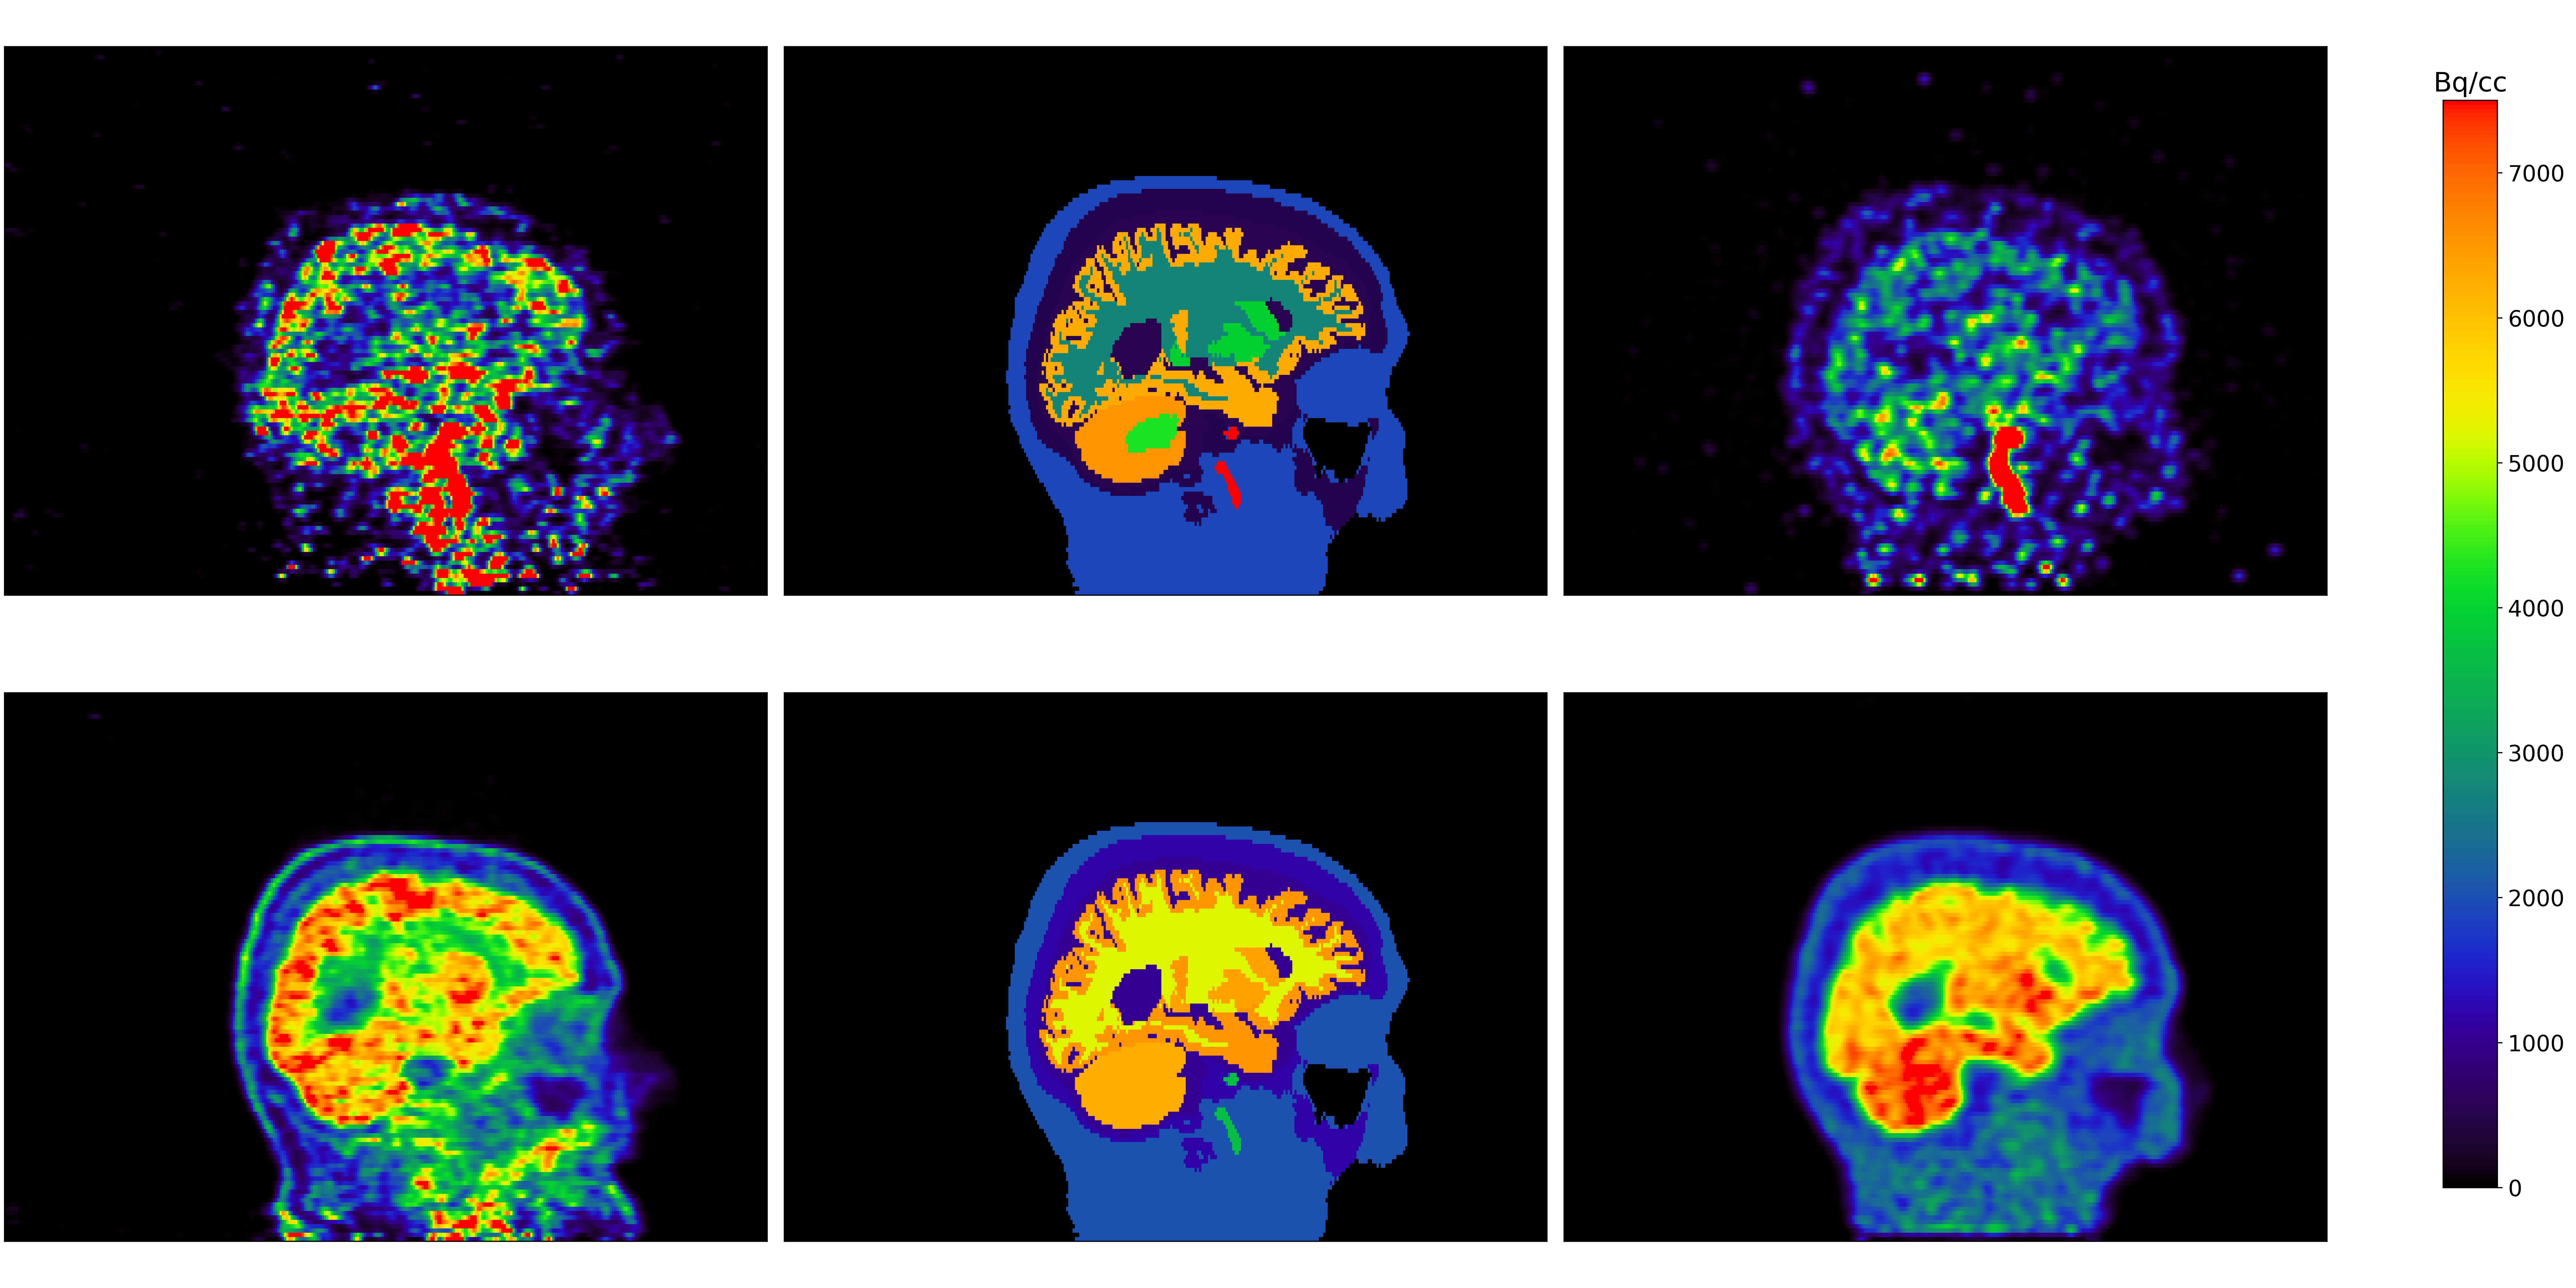
\includegraphics[width=\textwidth]{figures/sim_compare.jpg}

% gpt: make it in to figure and add appropriate caption ( its the comparison one)
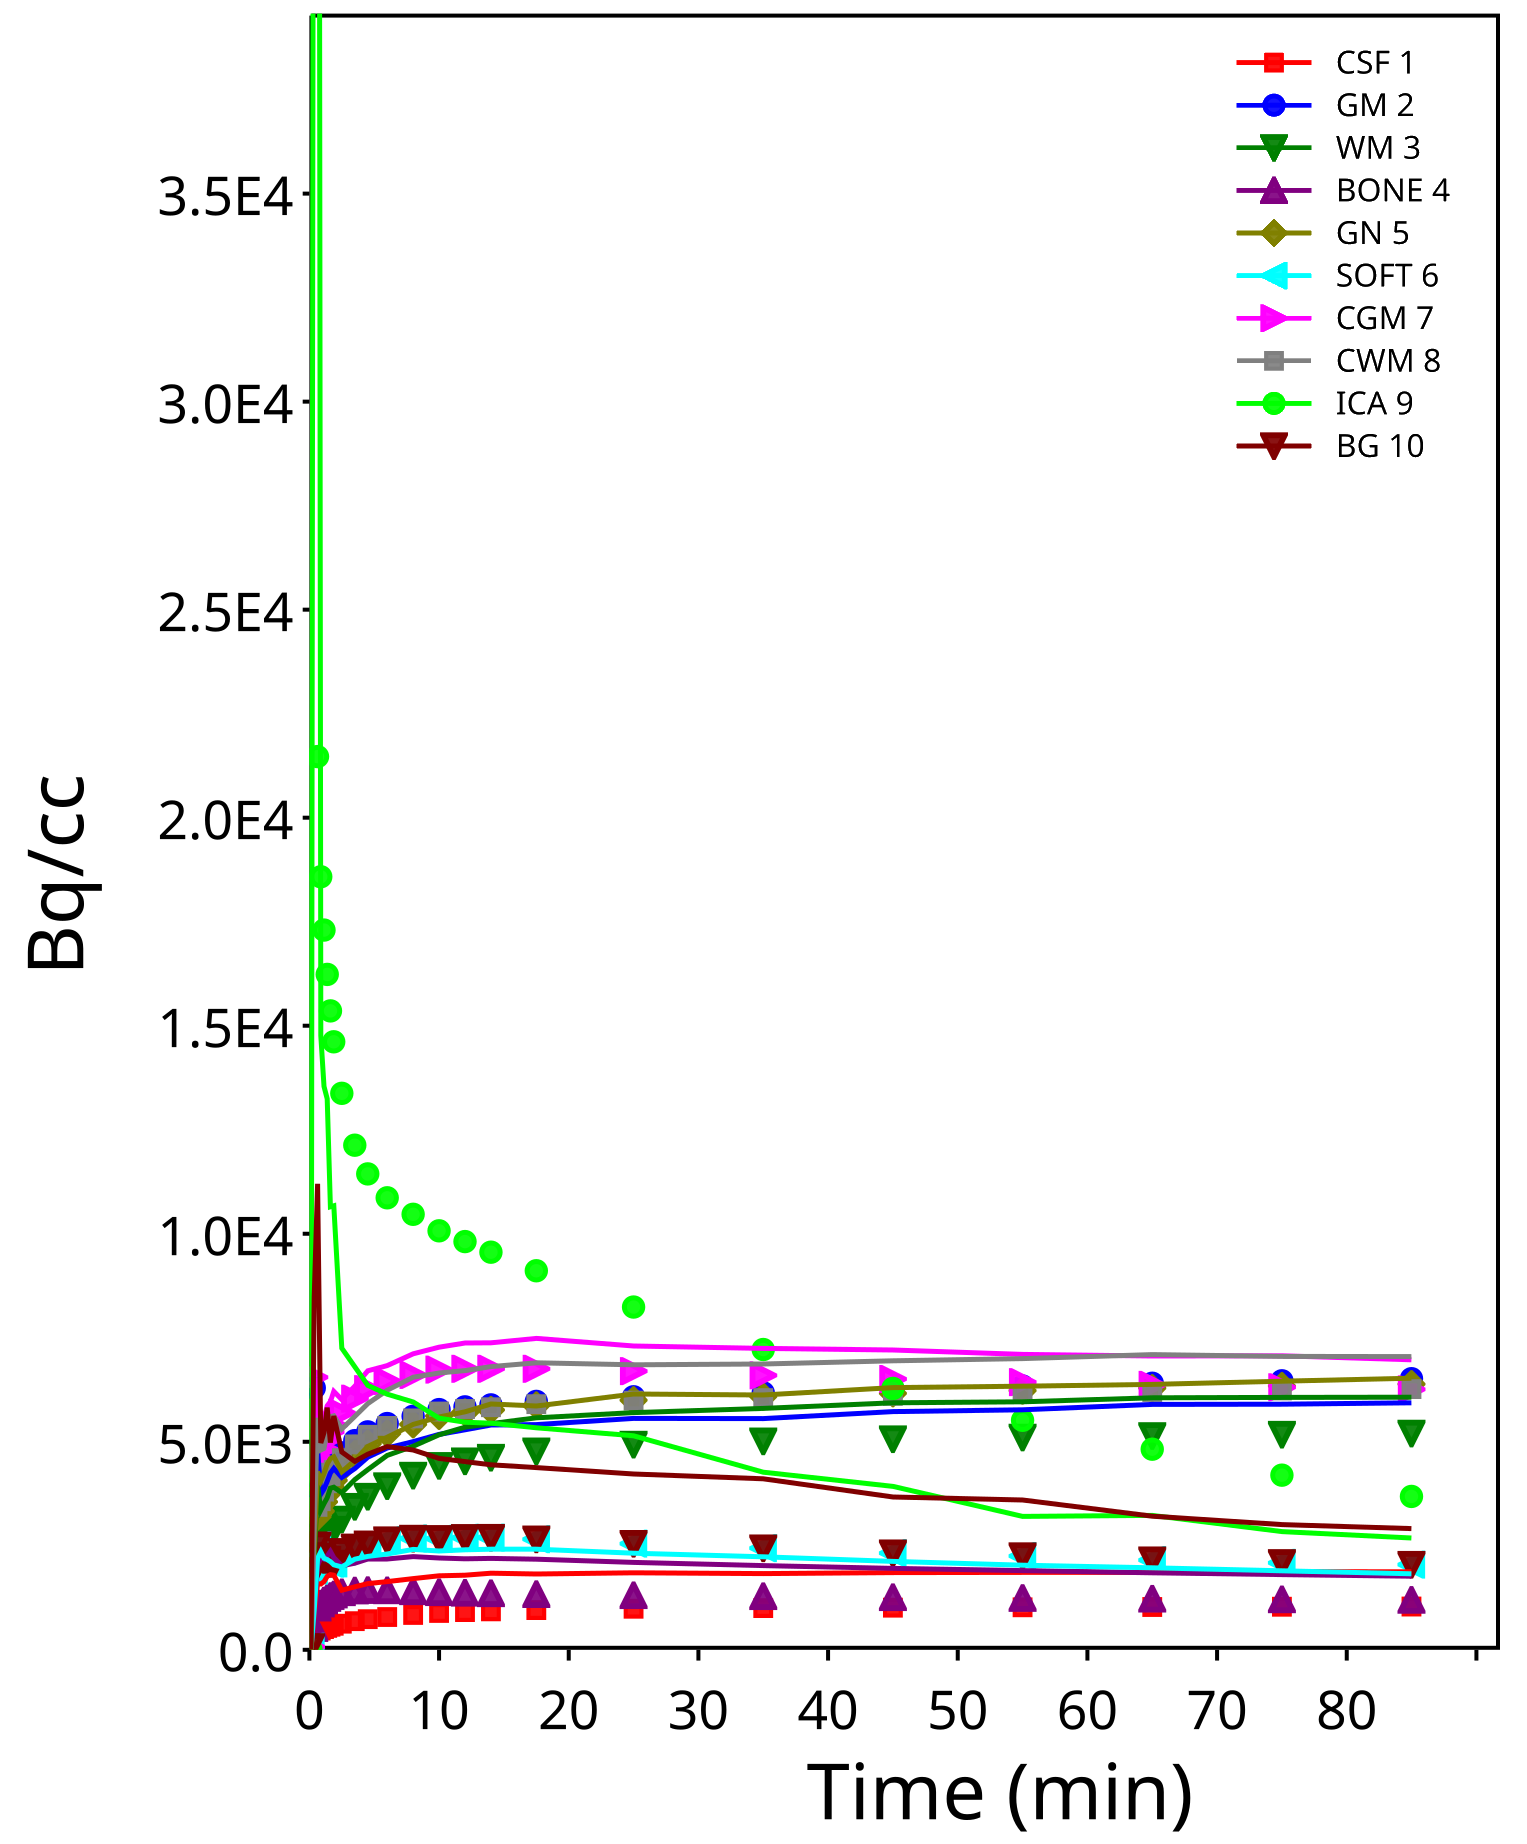
\includegraphics[width=0.6\textwidth]{figures/sim_tac.png}

\section{IDIF}

% GPT: fix sentencing and coherence
Since BGTM relies on the GTM method and also depends on a population AIF. Thus the performance should be compared compared to the IDIF derived from GTM method and also the Population Based Input Function (PBIF) which is the mean AIF used in the PCA (\(\mu_{IF}\)).
The Markov Chain was run for 230,000 iteration of which the first 30,000 were in the burn-in stage.

\subsection{\fdg\ Dataset}
% GPT: fix grammar issues and sentencing. don't change a lot
The reported statistic are from the experiment with the median results from the fine-tuning stage.

Figure~\ref{fig:fdg_ifs} compares the two methods for one of the best- and worst-performing subjects.
In the well-performing subject, BGTM significantly outperforms GTM and PBIF($\mrglu$ MAPE of 1.2\% vs. 26\% and 1.6\% respectively); however, in the poorly performing case, BGTM falls short of GTM and PBIF ($\mrglu$ MAPE of 36\% vs. 2.2\% and 4.75\% respectively).

\begin{figure}[h]
	\centering
	\begin{subfigure}[b]{0.322\textwidth}
		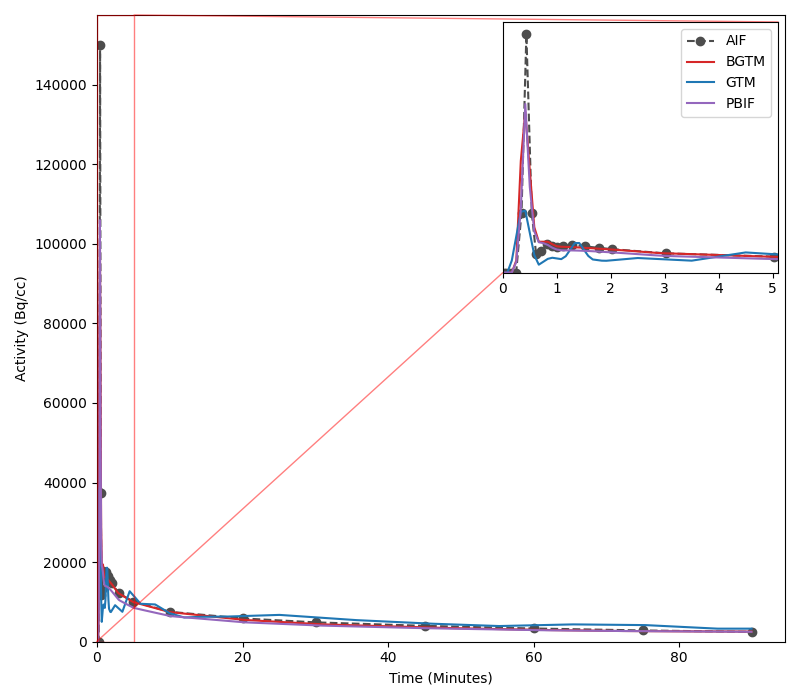
\includegraphics[width=\textwidth]{figures/PM10845_1_infunc.png}
		\caption{}
	\end{subfigure}
	\begin{subfigure}[b]{0.322\textwidth}
		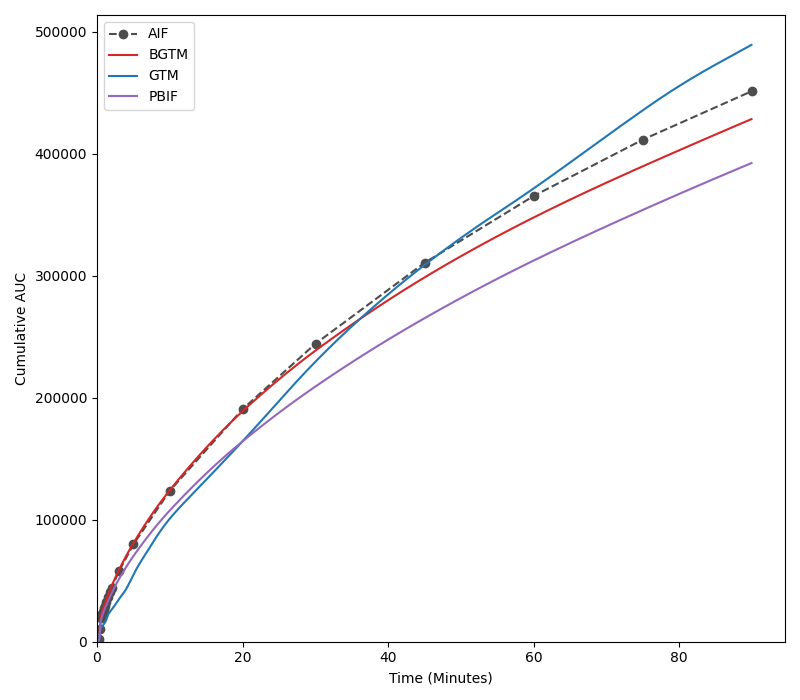
\includegraphics[width=\textwidth]{figures/PM10845_1_cauc.png}
		\caption{}
	\end{subfigure}
	\begin{subfigure}[b]{0.322\textwidth}
		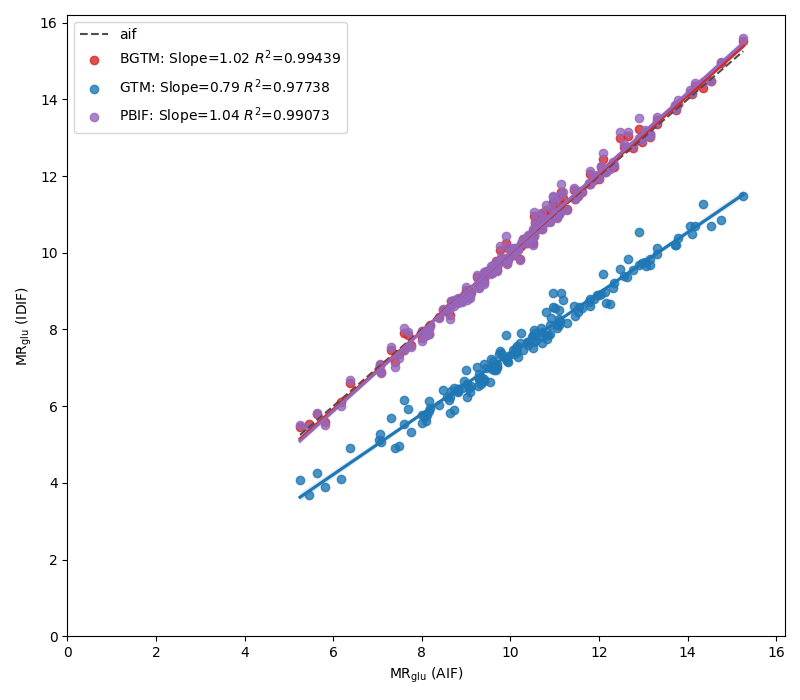
\includegraphics[width=\textwidth]{figures/PM10845_1_patlak_mrglu.png}
		\caption{}
	\end{subfigure}
	\begin{subfigure}[b]{0.322\textwidth}
		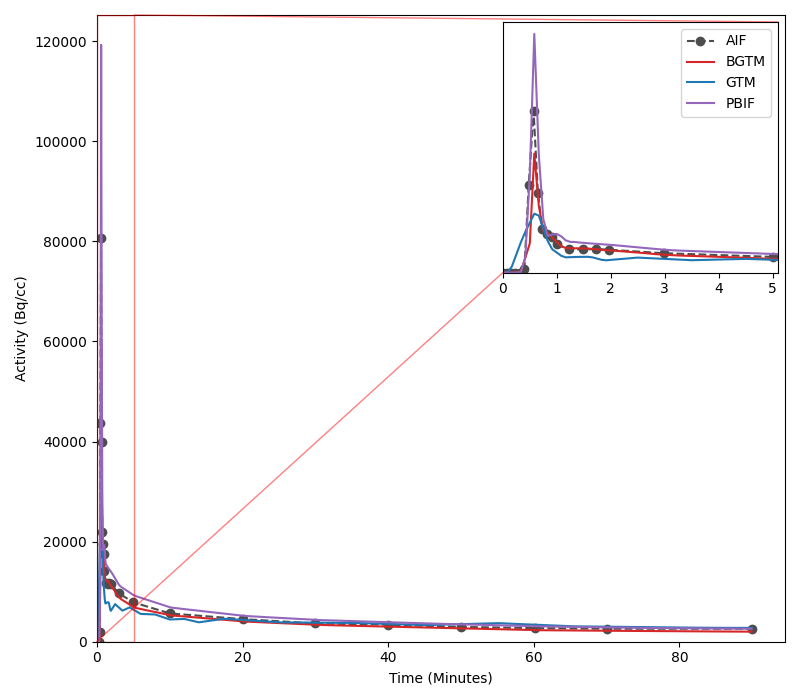
\includegraphics[width=\textwidth]{figures/COUJE07810_1_infunc.png}
		\caption{}
	\end{subfigure}
	\begin{subfigure}[b]{0.322\textwidth}
		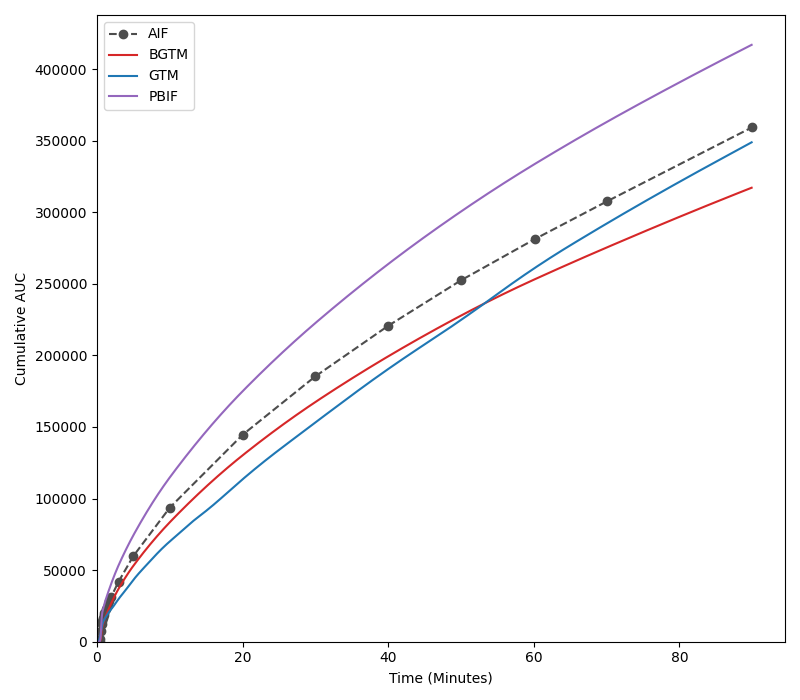
\includegraphics[width=\textwidth]{figures/COUJE07810_1_cauc.png}
		\caption{}
	\end{subfigure}
	\begin{subfigure}[b]{0.322\textwidth}
		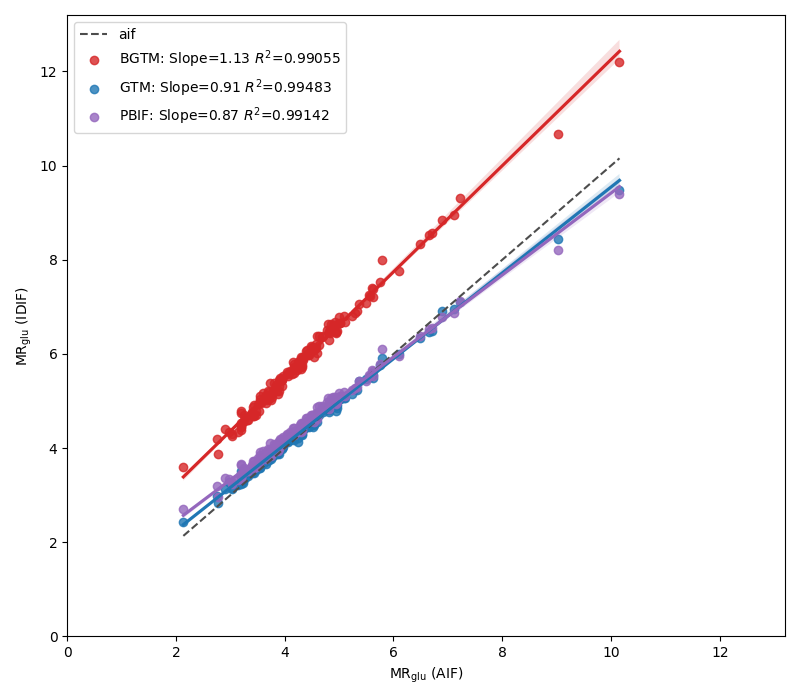
\includegraphics[width=\textwidth]{figures/COUJE07810_1_patlak_mrglu.png}
		\caption{}
	\end{subfigure}
	\caption{Comparison of the IFs (a,d), cumulative AUC curves (b,e), and $\mrglu$ regression lines (c,f) for one of the best-(top row) and worst-performing(bottom row) subjects in the \fdg\ dataset}
	\label{fig:fdg_ifs}
\end{figure}

The average mean absolute error of the cAUC curves across the dataset was 13,024 for BGTM and 15,709 and 14,630 for GTM and PBIF respectively (Figure~\ref{subfig:fdg_cauc_boxplot}).

In quantification BGTM resulted in better performance compared to GTM and PBIF methods.
Specifically, the BGTM, GTM, and PBIF methods achieved an average \(\mrglu\) mean absolute percentage error (MAPE) of 13\%, 24\%, 17\%, respectively (Figure~\ref{subfig:fdg_mape_boxplot}), and an average \(\mrglu\) MAE of 1.04, 1.98, and 1.4.
In addition, the MAPE for the coefficient of determination (\(R^2\)) and the regression slope (\(S\)) were 1.75\%, 11.2\% for BGTM, compared to 4.1\% and 17\% for GTM and 1.5\% and 15.75\% for PBIF, respectively.

\begin{figure}
	\centering
	\begin{subfigure}[b]{0.45\textwidth}
		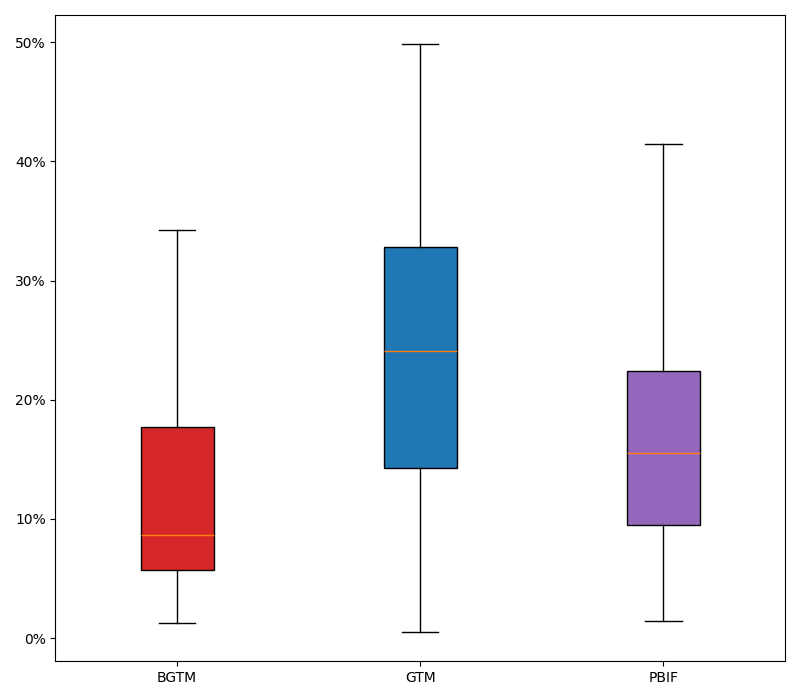
\includegraphics[width=\textwidth]{figures/fdg_quantification_patlak_mape_boxplot.png}
		\caption{\(\mrglu\) MAPE Boxplot}
		\label{subfig:fdg_mape_boxplot}
	\end{subfigure}
	\begin{subfigure}[b]{0.45\textwidth}
		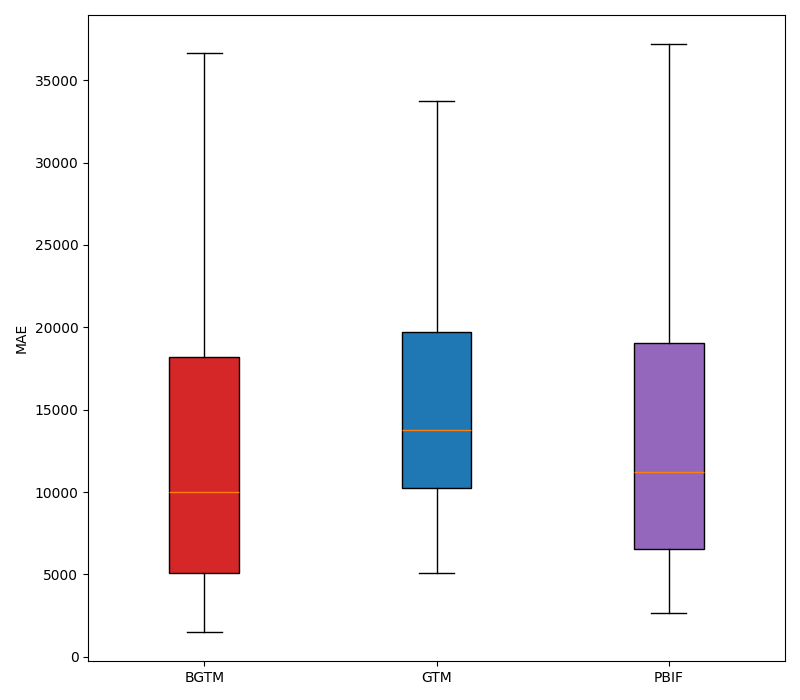
\includegraphics[width=\textwidth]{figures/fdg_curve_mae_boxplot.png}
		\caption{cAUC MAE Boxplot}
		\label{subfig:fdg_cauc_boxplot}
	\end{subfigure}
	\caption{Boxplot of curve and quantification errors for the \fdg\ dataset}
	\label{fig:fdg_boxplots}
\end{figure}




% GPT: dont touch
Paired t-tests were used to compare BGTM with GTM and PBIF on quantification metrics (Table~\ref{tab:metrics_all_fdg}).
Relative to GTM, BGTM showed significantly lower \(\mrglu\) MAE (\(t=-5.934, p=1.754\times 10^{-7}\)), \(\mrglu\) MAPE (\(t=-5.459,\,p=1.042\times 10^{-6}\)), \(R^2\) absolute percentage error (APE) (\(t=-2.762,\,p=7.677\times 10^{-3}\)), and slope APE (\(t=-4.030,\,p=1.644\times 10^{-4}\)).
Relative to PBIF, BGTM also yielded significantly lower \(\mrglu\) MAE (\(t=-2.974,\,p=4.275\times 10^{-3}\)), \(\mrglu\) MAPE (\(t=-2.415,\,p=1.890\times 10^{-2}\)), and slope APE (\(t=-3.036,\,p=3.583\times 10^{-3}\)), while the difference in \(R^2\) APE was not significant (\(t=1.680,\,p=9.832\times 10^{-2}\)).


\subsection{\yohimbine\ Dataset}

% GPT: fix grammar sentencing and coherence. should i keep the "it's mostly a lucky exception" or move it to discussion?
The success of the \fdg\ dataset was not able to be replicated for the \yohimbine\ dataset.
In Figure~\ref{fig:yoh_ifs} the best- and worst-performing subjects are compared.
However, the 5\% MAPE $V_T$ in the good performing subject cannot reliably be attributed to the well performance of the algorithm rather it's mostly a lucky exception.

Overall the average cAUC MAE of the dataset was 55{,}499 for BGTM and 96{,}362 and 37{,}613 for GTM and PBIF, respectively (Figure~\ref{subfig:yoh_cauc_boxplot}).
In quantification using Logan plot method, the average \(V_T\) MAPE was 75.9\%, 166.5\%, and 29.5\% for BGTM, GTM, and PBIF, respectively (Figure~\ref{subfig:yoh_mape_boxplot}).

As apparent by the Paired t-tests in Table~\ref{tab:metrics_all_yoh}, BGTM was able to perform better than GTM but performs significantly worst than the PBIF method.

\begin{figure}[p]
	\centering
	\begin{subfigure}[b]{0.322\textwidth}
		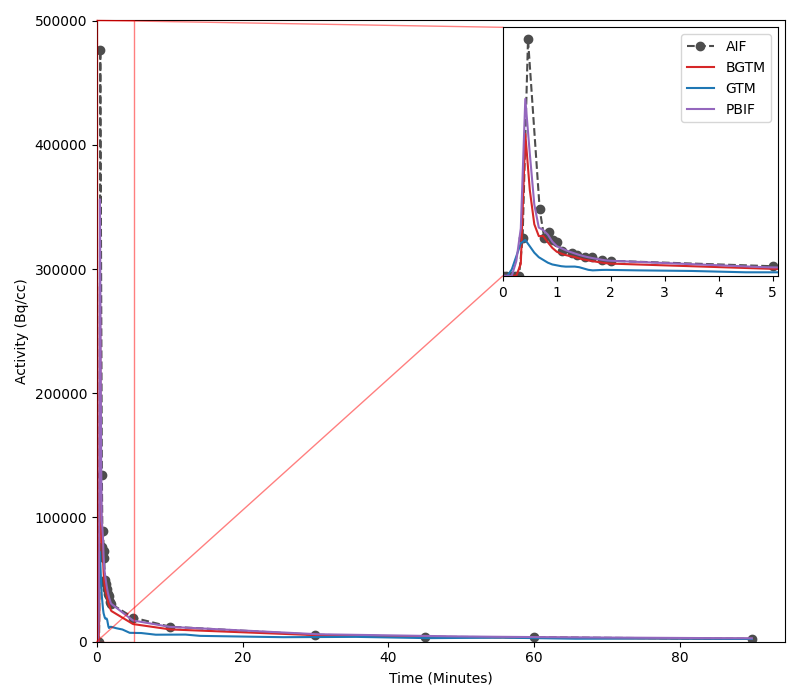
\includegraphics[width=\textwidth]{figures/LUCAU08056_TEST_infunc.png}
		\caption{}
	\end{subfigure}
	\begin{subfigure}[b]{0.322\textwidth}
		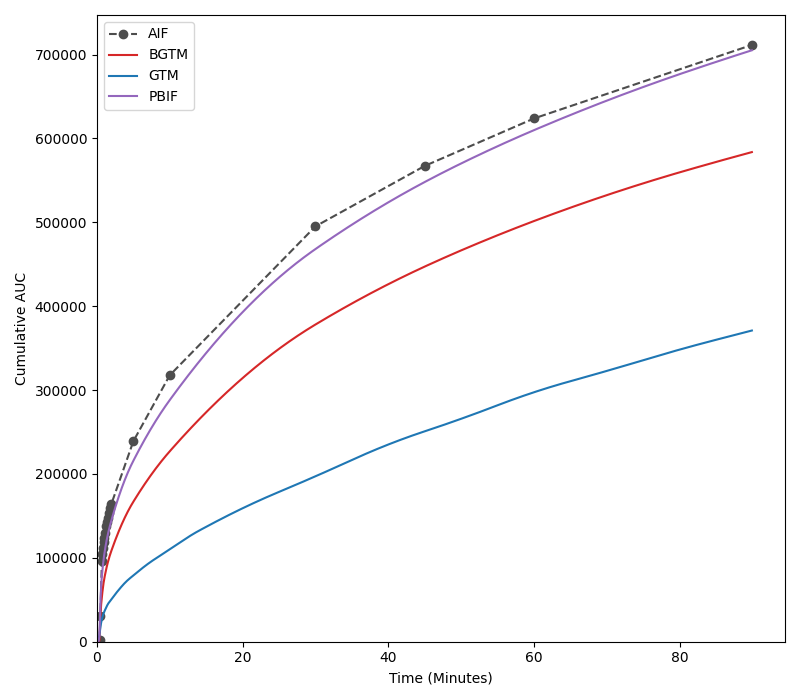
\includegraphics[width=\textwidth]{figures/LUCAU08056_TEST_cauc.png}
		\caption{}
	\end{subfigure}
	\begin{subfigure}[b]{0.322\textwidth}
		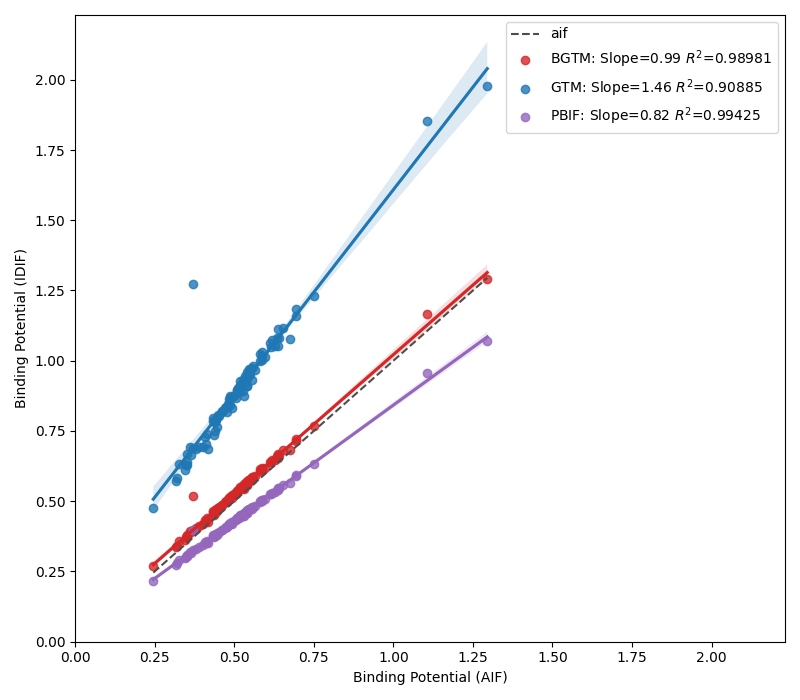
\includegraphics[width=\textwidth]{figures/LUCAU08056_TEST_logan_bp.png}
		\caption{}
	\end{subfigure}
	\begin{subfigure}[b]{0.322\textwidth}
		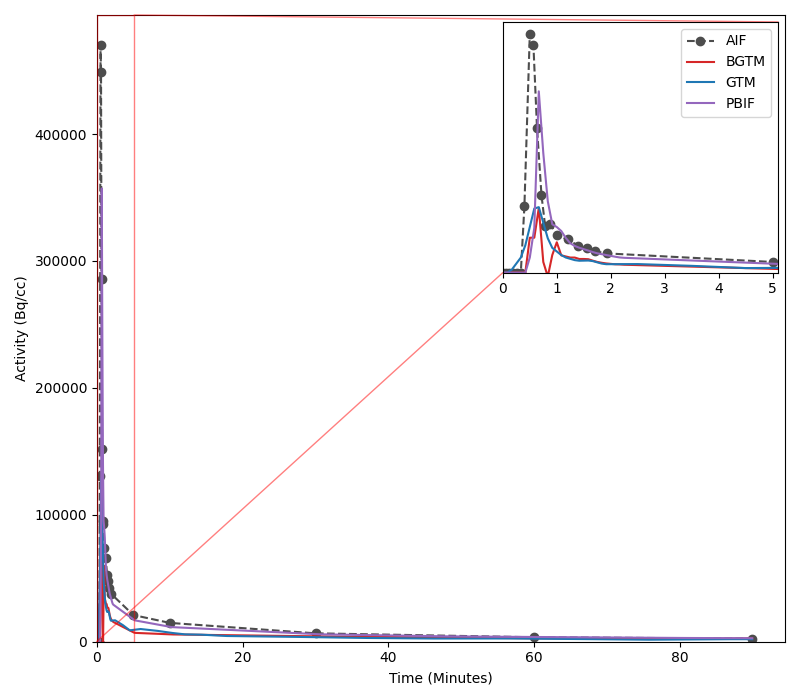
\includegraphics[width=\textwidth]{figures/GOIAX07977_TEST_infunc.png}
		\caption{}
	\end{subfigure}
	\begin{subfigure}[b]{0.322\textwidth}
		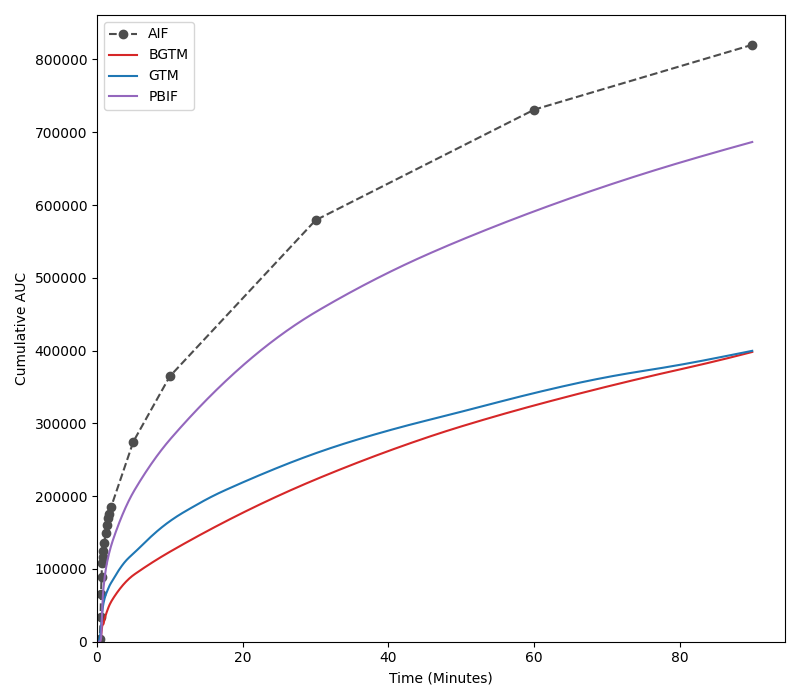
\includegraphics[width=\textwidth]{figures/GOIAX07977_TEST_cauc.png}
		\caption{}
	\end{subfigure}
	\begin{subfigure}[b]{0.322\textwidth}
		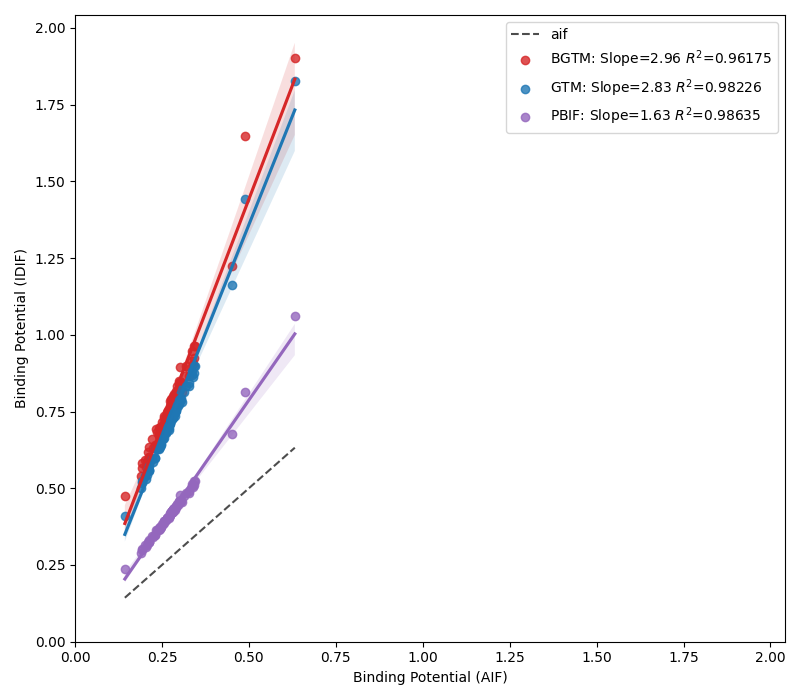
\includegraphics[width=\textwidth]{figures/GOIAX07977_TEST_logan_bp.png}
		\caption{}
	\end{subfigure}
	\caption{Comparison of the IFs (a,d), cumulative AUC curves (b,e), and $V_T$ regression lines (c,f) for one of the best-(top row) and worst-performing(bottom row) subjects in the \yohimbine\ dataset}
	\label{fig:yoh_ifs}
\end{figure}

\begin{figure}[p]
	\centering
	\begin{subfigure}[b]{0.45\textwidth}
		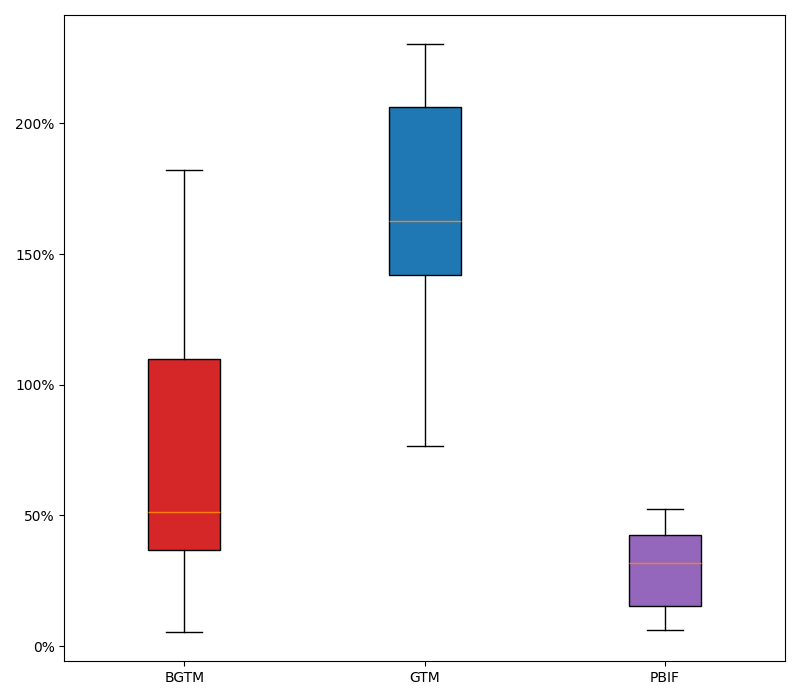
\includegraphics[width=\textwidth]{figures/yoh_quantification_logan_mape_boxplot.png}
		\caption{\(\mrglu\) MAPE Boxplot}
		\label{subfig:yoh_mape_boxplot}
	\end{subfigure}
	\begin{subfigure}[b]{0.45\textwidth}
		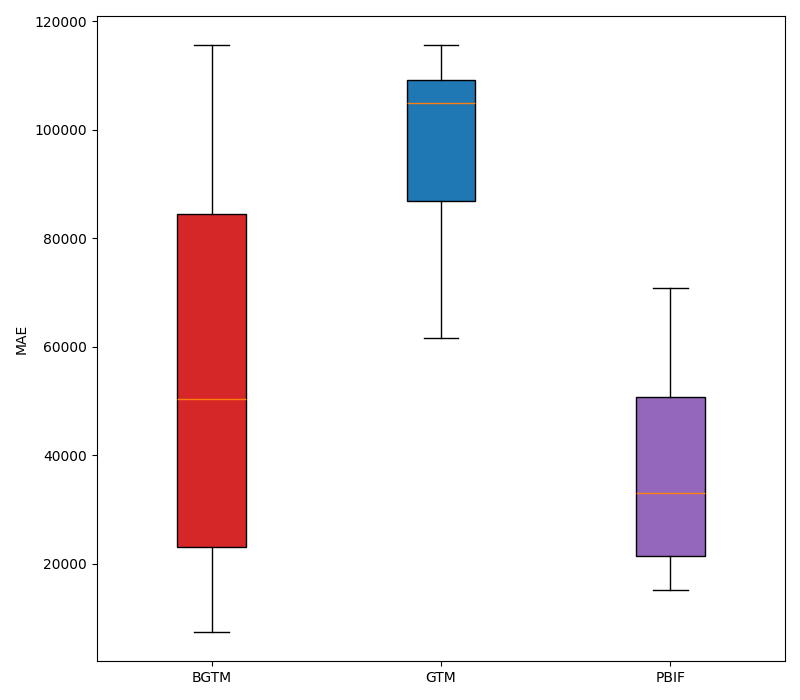
\includegraphics[width=\textwidth]{figures/yoh_curve_mae_boxplot.png}
		\caption{cAUC MAE Boxplot}
		\label{subfig:yoh_cauc_boxplot}
	\end{subfigure}
	\caption{Boxplot of curve and quantification errors of the \yohimbine\ dataset}
	\label{fig:yoh_boxplots}
\end{figure}


% GPT: Don't touch tables
\begin{sidewaystable}[b]
	\centering
	\small
	\setlength{\tabcolsep}{10pt}
	\begin{tabular}{l|cc|cc|cc|cc|cc}
		\toprule
		\multirow{2}{*}{\textbf{Metric}} & \multicolumn{2}{c|}{\textbf{BGTM}} & \multicolumn{2}{c|}{\textbf{GTM}} & \multicolumn{2}{c|}{\textbf{PBIF}} & \multicolumn{2}{c|}{\textbf{BGTM vs GTM}} & \multicolumn{2}{c}{\textbf{BGTM vs PBIF}}                                                                                                                  \\
		\cmidrule(lr){2-3} \cmidrule(lr){4-5} \cmidrule(lr){6-7} \cmidrule(lr){8-9} \cmidrule(lr){10-11}
		                                 & \(\mu\)                            & \(\sigma\)                        & \(\mu\)                            & \(\sigma\)                                & \(\mu\)                                   & \(\sigma\) & \(t\)      & \(p\)                              & \(t\)      & \(p\)                              \\
		\midrule
		IF cAUC MAE                      & 13{,}024                           & 10{,}410                          & 15{,}709                           & 7{,}884                                   & 14{,}630                                  & 10{,}268   & \(-2.388\) & \(2.023\times 10^{-2}\) \sym{*}    & \(-1.278\) & \(2.065\times 10^{-1}\)            \\
		IF cAUC RMSE                     & 20{,}293                           & 16{,}078                          & 23{,}380                           & 11{,}979                                  & 23{,}334                                  & 16{,}803   & \(-1.907\) & \(6.151\times 10^{-2}\) \sym{\dag} & \(-1.439\) & \(1.555\times 10^{-1}\)            \\
		IF AUC APE (\%)                  & 11.93                              & 10.76                             & 11.57                              & 11.50                                     & 14.34                                     & 11.08      & \(0.297\)  & \(7.674\times 10^{-1}\)            & \(-1.862\) & \(6.767\times 10^{-2}\) \sym{\dag} \\
		\midrule
		\(\mrglu\) MAPE (\%)             & 13.19                              & 10.57                             & 24.36                              & 13.68                                     & 17.17                                     & 12.41      & \(-5.459\) & \(1.042\times 10^{-6}\) \sym{***}  & \(-2.415\) & \(1.890\times 10^{-2}\) \sym{*}    \\
		\(\mrglu\) MAE                   & 1.04                               & 0.92                              & 1.98                               & 1.33                                      & 1.40                                      & 1.10       & \(-5.934\) & \(1.754\times 10^{-7}\) \sym{***}  & \(-2.974\) & \(4.275\times 10^{-3}\) \sym{**}   \\
		\(R^2\) APE (\%)                 & 1.76                               & 4.07                              & 4.13                               & 8.90                                      & 1.50                                      & 3.53       & \(-2.762\) & \(7.677\times 10^{-3}\) \sym{**}   & \(1.680\)  & \(9.832\times 10^{-2}\)            \\
		Slope APE (\%)                   & 11.28                              & 9.37                              & 17.05                              & 10.58                                     & 15.76                                     & 11.41      & \(-4.030\) & \(1.644\times 10^{-4}\) \sym{***}  & \(-3.036\) & \(3.583\times 10^{-3}\) \sym{**}   \\
		\bottomrule
	\end{tabular}
	\caption{Comprehensive curve and quantification metrics for the \fdg\ dataset.
		Values are means (\(\mu\)) and standard deviations (\(\sigma\)) across subjects.
		Paired two-sided \(t\)-tests compare GTM or PBIF against BGTM for each metric.
		Significance codes: \sym{*}\,p<0.05, \sym{**}\,p<0.01, \sym{***}\,p<0.001, \sym{\dag}\,p<0.10 (trend).}

	\label{tab:metrics_all_fdg}
\end{sidewaystable}
\begin{sidewaystable}[b]
	\centering
	\small
	\setlength{\tabcolsep}{10pt}
	\begin{tabular}{l|cc|cc|cc|cc|cc}
		\toprule
		\multirow{2}{*}{\textbf{Metric}} & \multicolumn{2}{c|}{\textbf{BGTM}} & \multicolumn{2}{c|}{\textbf{GTM}} & \multicolumn{2}{c|}{\textbf{PBIF}} & \multicolumn{2}{c|}{\textbf{BGTM vs GTM}} & \multicolumn{2}{c}{\textbf{BGTM vs PBIF}}                                                                                                  \\
		\cmidrule(lr){2-3} \cmidrule(lr){4-5} \cmidrule(lr){6-7} \cmidrule(lr){8-9} \cmidrule(lr){10-11}
		                                 & \(\mu\)                            & \(\sigma\)                        & \(\mu\)                            & \(\sigma\)                                & \(\mu\)                                   & \(\sigma\) & \(t\)      & \(p\)                          & \(t\)      & \(p\)                  \\
		\midrule
		IF cAUC MAE                      & 55{,}499                           & 40{,}271                          & 96{,}362                           & 20{,}343                                  & 37{,}613                                  & 20{,}456   & \(-3.404\) & \(1.443\times10^{-2}\)\sym{*}  & \(0.959\)  & \(3.748\times10^{-1}\) \\
		IF cAUC RMSE                     & 83{,}282                           & 60{,}130                          & 147{,}032                          & 28{,}318                                  & 52{,}313                                  & 27{,}845   & \(-3.789\) & \(9.083\times10^{-3}\)\sym{**} & \(1.196\)  & \(2.768\times10^{-1}\) \\
		IF AUC APE (\%)                  & 26.14                              & 19.02                             & 52.75                              & 3.53                                      & 17.74                                     & 14.78      & \(-3.644\) & \(1.078\times10^{-2}\)\sym{*}  & \(0.872\)  & \(4.168\times10^{-1}\) \\
		\midrule
		\(V_T\) MAPE (\%)                & 75.91                              & 62.09                             & 166.48                             & 52.91                                     & 29.47                                     & 17.73      & \(-3.628\) & \(1.100\times10^{-2}\)\sym{*}  & \(2.588\)  & \(4.133\times10^{-2}\) \\
		\(V_T\) MAE                      & 0.324                              & 0.211                             & 0.812                              & 0.360                                     & 0.132                                     & 0.072      & \(-3.477\) & \(1.318\times10^{-2}\)\sym{*}  & \(3.042\)  & \(2.275\times10^{-2}\) \\
		\(R^2\) APE (\%)                 & 2.04                               & 1.83                              & 2.27                               & 3.09                                      & 2.06                                      & 2.40       & \(-0.148\) & \(8.870\times10^{-1}\)         & \(-0.040\) & \(9.692\times10^{-1}\) \\
		Slope APE (\%)                   & 81.18                              & 68.33                             & 161.80                             & 73.59                                     & 35.06                                     & 24.22      & \(-3.167\) & \(1.939\times10^{-2}\)\sym{*}  & \(2.409\)  & \(5.263\times10^{-2}\) \\
		\bottomrule
	\end{tabular}
	\caption{Comprehensive curve and quantification metrics for the \yohimbine\ dataset.
		Values are means (\(\mu\)) and standard deviations (\(\sigma\)) across subjects.
		Paired two-sided \(t\)-tests compare GTM or PBIF against BGTM for each metric.
		Significance codes: \sym{*}\,p<0.05, \sym{**}\,p<0.01, \sym{***}\,p<0.001, \sym{\dag}\,p<0.10 (trend).}
	\label{tab:metrics_all_yoh}
\end{sidewaystable}

\subsection{Simulated Dataset}

As a complementary quality control step, the performance of Direct IDIF (meaning with no PVC) of the experimental dataset was compared to the simulated dataset.
The average cAUC MAE of the experimental dataset was 34,929 compared to 
